
\documentclass[%
 reprint,
superscriptaddress,
%groupedaddress,
%unsortedaddress,
%runinaddress,
%frontmatterverbose, 
%preprint,
%preprintnumbers,
%nofootinbib,
%nobibnotes,
%bibnotes,
 amsmath,amssymb,
 aps,
%pra,
%prb,
%rmp,
%prstab,
%prstper,
floatfix,
]{revtex4-2}

\usepackage{graphicx}% Include figure files
\usepackage{dcolumn}% Align table columns on decimal point
\usepackage{xcolor}
\usepackage{bm}% bold math
%\usepackage{hyperref}% add hypertext capabilities
%\usepackage[mathlines]{lineno}% Enable numbering of text and display math
%\linenumbers\relax % Commence numbering lines

%\usepackage[showframe,%Uncomment any one of the following lines to test 
%%scale=0.7, marginratio={1:1, 2:3}, ignoreall,% default settings
%%text={7in,10in},centering,
%%margin=1.5in,
%%total={6.5in,8.75in}, top=1.2in, left=0.9in, includefoot,
%%height=10in,a5paper,hmargin={3cm,0.8in},
%]{geometry}

\begin{document}

\title{Modeling the Spread of Ebola in West Africa} % Force line breaks with \\

\author{Jason Hunter}
% UNCOMMENT THIS IF YOU HAVE A SECOND AUTHOR
% \author{Second Author}


\date{December 15, 2024}% It is always \today, today,
             %  but any date may be explicitly specified

\begin{abstract}
{\bf Abstract:} \textcolor{blue}{
    For this project, I designed and created a standard SIR model using python to simulate the spread of Ebola in a population. 
    From this, I created a modified model in an attempt to tune the model to Ebola specific dynamics. 
    This model accounted for an additional population of 'exposed' individuals, which made it possible to take into account the latency period of Ebola. 
    Finally, I added a quarantine parameter to the model to simulate the effects of containment on the spread of the disease. 
    The model was then used to simulate the spread of Ebola in West Africa using a mixture of both mock data and real metrics gathered from various datasets. 
    I then attempt to do a more geospatial analysis of the epidemic as it took place in West Africa.}
\end{abstract}

\maketitle

\section{Introduction and Background}

\textcolor{blue}{ 
    Ebola virus disease (EVD) is a highly lethal viral hemmorhagic fever which has caused several widespread outbreaks in Africa.
    It was first discovered in 1976 when two outbreaks occurred in Sudan and the Democratic Republic of Congo near the Ebola river, debuting the disease's name.
    Since then the disease has caused several outbreaks in Africa, with the most severe being the 2014-2016 outbreak. 
    The virus is zoonotic in nature, meaning that it spreads from wild animals to humans [2].
    It is widely believed that fruit bats are the source of the virus, and may have been sold as bushmeat at local markets. 
    The virus then spreads through human-to-human contact, and can be spread through bodily fluids, blood, and other secretions. 
    The virus has an incubation period in the range of 2-21 days, and symptoms include fever, muscle pain, fatigue, headache, and sore throat [3].
    These symptoms are then followed by vomiting, diarrhea, rash, and in some cases, internal and external bleeding [3].
    The disease has a high mortality rate, with the 2014-2016 outbreak in West Africa having an average mortality rate of around 40\%, resulting in around 11,000 deaths out of about 28,000 cases across Sierra Leone, Liberia, and Guinea.}

\textcolor{blue}{
    A common model used in the simulation of infectious disease spread is the SIR model. 
    This model separates the population into three distinct compartments: Susceptible, Infected, and Recovered. 
    A set of differential equations is then used to model the flow of individuals between these populations with respect to time. 
    A common extension to the SIR model is the SEIRD model, which adds two additional compartments for Exposed and Deceased individuals. 
    The Exposed compartment accounts for the latency period of the disease, where individuals are infected but not yet infectious. 
    This is especially useful for diseases such as Ebola, which have an extensive latent period. 
    The Deceased compartment accounts for individuals who have died from the disease.
    When combined with realistic disease parameters and population data, these models can be used to simulate the spread of infectious diseases and predict the effects of various interventions.}

\textcolor{blue}{
    In my project, I've used a modified SEIRD model in an attempt to run simulations of the spread of Ebola in West Africa.
    My modifications to the model include the addition of a containment parameter, which effectively acts as a quarantine for infected people. 
    Alongside this, I've also added an effectiveness rate to the containment parameter, which allows for the simulation of different levels of containment. 
    With this I hope to better understand how a combination of both rapid and effective containment procedures can help to mitigate the spread of contagious disease.}

\textcolor{blue}{I've also gathered data from a variety of sources, including the World Health Organization (WHO), the Centers for Disease Control and Prevention (CDC), as well as a few githubs. 
This data includes Ebola specific disease metrics, as well as coordinates of the affected areas,
which I then use to attempt a geospatial analysis of the epidemic as it took place in West Africa.}

\section{Learning Goals}

\textcolor{blue}{
    My main learning goal for this project was to model the spread of the Ebola epidemic in West African countries using an SEIRD framework and to understand how containment measures could have affected the spread of the disease. 
    I aimed to use this SEIRD model to visualize the spread of the disease in a way that would be easy to understand and interpret.
    I wanted to gain a better understanding of how these models work, and how they are used to represent real-world disease dynamics.}

\textcolor{blue}{
    I also gained vital experience in both data collection and analysis during this project. 
    It was important to source data from several places, and to understand the importance of using clean and reliable data. 
    I also learned how to use this data to create visualizations that could help to better understand the spread of the disease. 
    This continued to excel my skills in Python and data analysis.
    I learned how to use geospatial data to create maps of the epidemic, and how to use these maps to better understand the spread of it. 
    This was a new skill for me, and I found it to be very interesting and useful.}

\section{Findings and Results}

\begin{figure}[t]
    \centering
    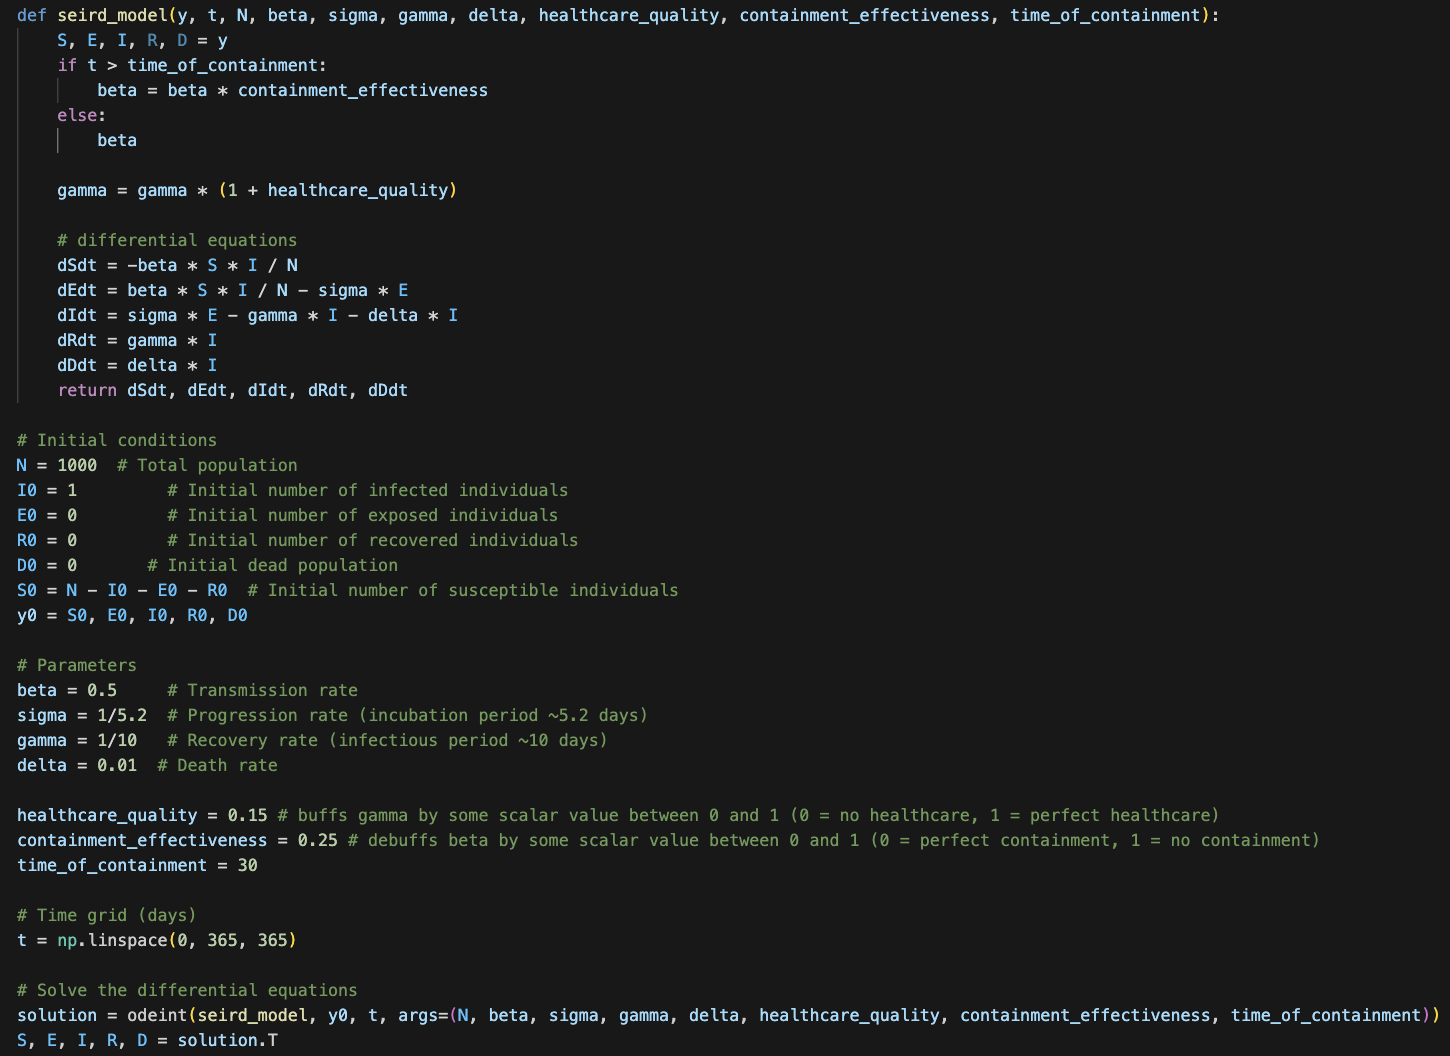
\includegraphics[width=0.5\textwidth]{SEIRD Model.png}
    \caption{Python code for the SEIRD model used in this project.}
    \label{SEIRD Model}
\end{figure}

\textcolor{blue}{Using the SEIRD model depicted in Figure \ref{SEIRD Model}, I was able to run theoretical simulations of the spread of Ebola in West Africa.
I included key parameters that are a part of all SEIRD models, 
such as the transmission rate $\beta$, which dictates the rate at which susceptible individuals become infected, 
the rate of recovery $\gamma$, which is the rate at which infectious individuals recover, 
as well as the incubation rate $\sigma$, which is indicative of the rate at which exposed individuals become infectious.
I also include a death rate $\delta$, which is the rate at which infected individuals die.
This is an important parameter for diseases such as Ebola, which have a high mortality rate.
Lastly, I included two parameters for containment: the date at which containment measures were implemented, and the effectiveness of these measures.}
\textcolor{blue}{The SEIRD equations used in the model are as follows:
\begin{equation}
    \frac{dS}{dt} = -\beta \frac{S}{N} I
    \label{dSdt}
\end{equation}
\begin{equation}
    \frac{dE}{dt} = \beta \frac{S}{N} I - \sigma E
    \label{dEdt}
\end{equation}
\begin{equation}
    \frac{dI}{dt} = \sigma E - \gamma I - \delta I
    \label{dIdt}
\end{equation}
\begin{equation}
    \frac{dR}{dt} = \gamma I
    \label{dRdt}
\end{equation}
\begin{equation}
    \frac{dD}{dt} = \delta I
    \label{dDdt}
\end{equation}
where $S$ is the number of susceptible individuals, 
$E$ is the number of exposed individuals, 
$I$ is the number of infected individuals, 
$R$ is the number of recovered individuals, 
$D$ is the number of deceased individuals, 
$N$ is the total population, 
$\beta$ is the transmission rate, 
$\sigma$ is the incubation rate, 
$\gamma$ is the recovery rate, 
and $\delta$ is the death rate.}

\textcolor{blue}{
    At this point I ran several simulations to try to understand how turning these various knobs on the model would affect the spread of the disease.
    The first one I ran was a base model with no healthcare or containment measures in place.
    The disease is effectively allowed to spread unchecked throughout the population.
    The total death count at the end of the base run was 31.
    I used this death toll as a baseline to compare the effectiveness of healthcare and containment measures I would test in further simulations.}
\begin{figure}[hbt!]
    \centering
    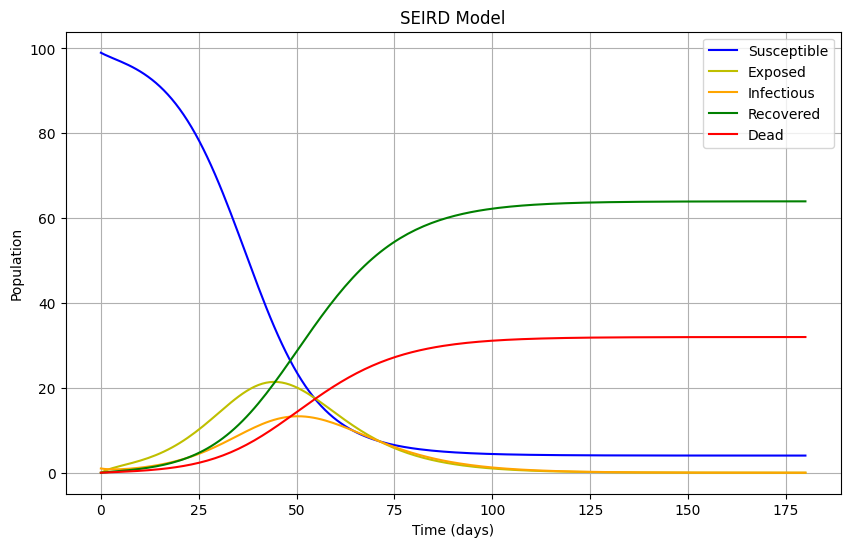
\includegraphics[width=0.5\textwidth]{BaseModel.png}
    \caption{Base Model Simulation.}
    \label{Base Model}
\end{figure}
\subsection{Impact of Healthcare Quality}
\textcolor{blue}{
    An additional parameter I attempted to account for in my model was the quality of healthcare in the affected areas. 
    I added healthcare quality, which was represented as a proportion from 0 to 1, in which 0 represented no healthcare at all and 1 represented the best healthcare possible. 
    This was multiplied by the recovery rate $\gamma$ to simulate the effects of healthcare on the recovery of infected individuals.
    In this simulation, I used a 
    healthcare quality of 0.5, 
    a transmission rate of 0.4,
    a recovery rate of 0.1, 
    an incubation rate of 0.1, 
    and a death rate of 0.05, 
    an initial population $N$ of 100,
    an initial number of infected individuals $I$ of 1, 
    and all other initial compartments set to 0. 
    Additionally, I set the containment effectiveness to 0.5, 
    and the containment date to 30 days after the start of the simulation which runs for a total of 180 days. }
\begin{figure}[hbt!]
    \centering
    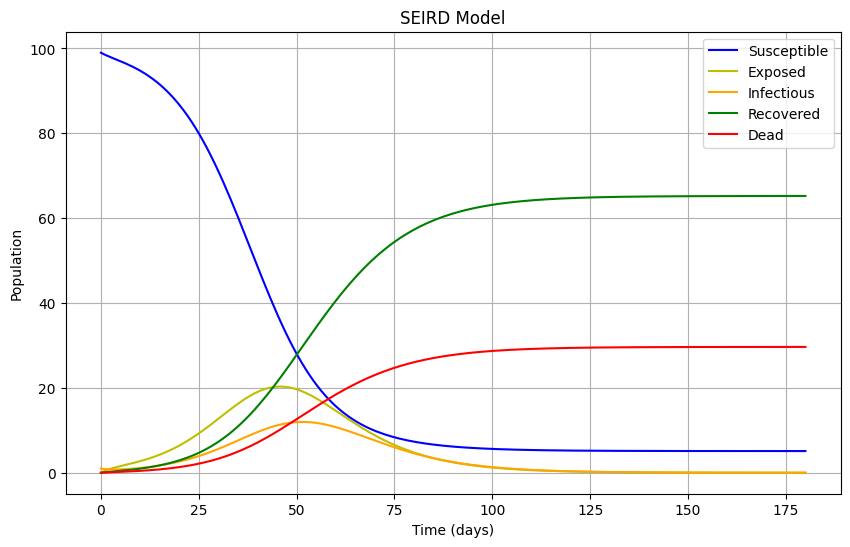
\includegraphics[width=0.5\textwidth]{HealthCareA.png}
    \caption{Simulation w/ Healthcare Quality = 0.1.}
    \label{HealthcareA}
\end{figure}
\begin{figure}[hbt!]
    \centering
    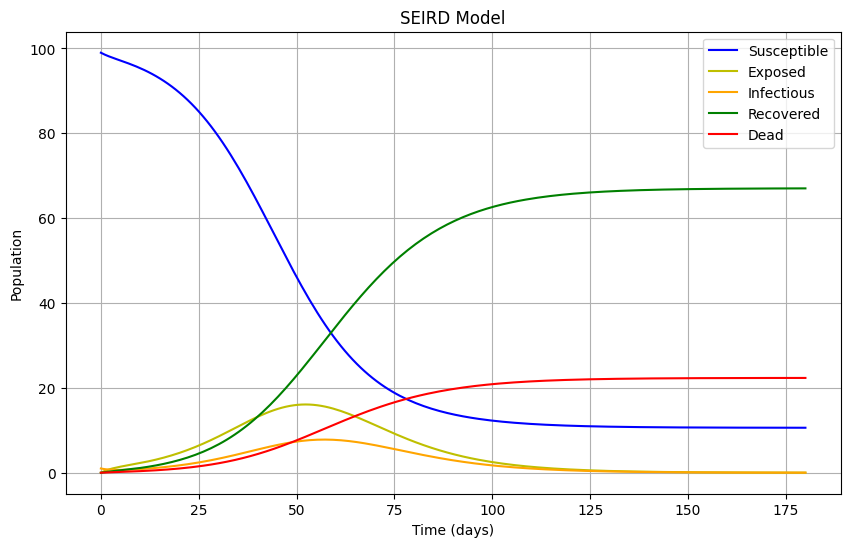
\includegraphics[width=0.5\textwidth]{HealthCareB.png}
    \caption{Simulation w/ Healthcare Quality = 0.5.}
    \label{HealthcareB}
\end{figure}
\begin{figure}[hbt!]
    \centering
    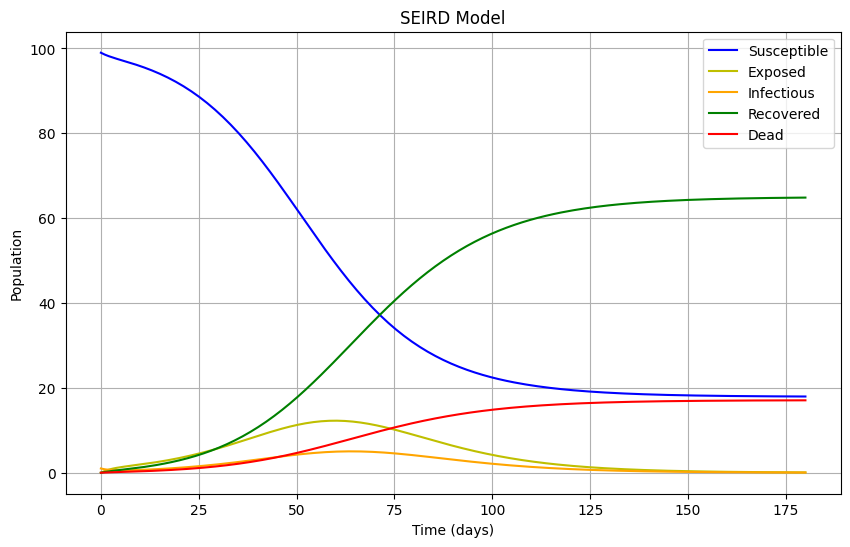
\includegraphics[width=0.5\textwidth]{HealthCareC.png}
    \caption{Simulation w/ Healthcare Quality = 0.9.}
    \label{HealthcareC}
\end{figure} \\
\textcolor{blue}{
In the model, I found that the quality of healthcare had a significant impact on the spread of the disease. 
In simulations with poor healthcare set to 0.1, the disease spread more rapidly and had a higher mortality rate (deaths = 29). 
In simulations with better healthcare set to 0.5, the disease spread more slowly and had a lower mortality rate (deaths = 22).
In simulations with better healthcare set to 0.9, the disease spread more slowly and had a lower mortality rate (deaths = 17). 
This highlights the importance of quality healthcare in controlling the spread of disease.}
\textcolor{blue}{
   In figures 2, 3, and 4, I show the results of the simulations with different levels of healthcare quality.
   When healthcare quality is high (figure 3), the disease spreads more slowly and has a lower mortality rate. 
   When healthcare quality is average (figure 4), and the final death count is 22.
   When healthcare quality is low (figure 5), the disease seems to spread more rapidly and has a higher mortality rate with a final death count of 29.}
\subsection{Impact of Containment Measures}
\textcolor{blue}{
    I also ran simulations to understand the impact of containment measures on the spread of the disease. 
    I used the same parameters as in the previous simulation, but changed the containment effectiveness to 0.9, and the containment date to 30 days after the start of the simulation.
    I also reset there to be no healthcare quality in this simulation to keep my results consistent.
    In the simulation with low containment effectiveness (figure 6),  the disease spread still spread fairly quickly and had a high mortality rate (deaths = 31)
    When containment effectiveness was average (figure 7), mortality rate decreased in comparison to the previous simulation (deaths = 25).
    When containment effectiveness was high (figure 8), the disease spread most slowly and had a lower mortality rate (deaths = 12).
    The graph in figure 8 shows the most effective containment measures, where the disease is effectively stopped in its tracks.
    This gives rise to the importance of implementing effective containment measures to control the spread of ebola and other diseases.}

\begin{figure}[hbt!]
    \centering
    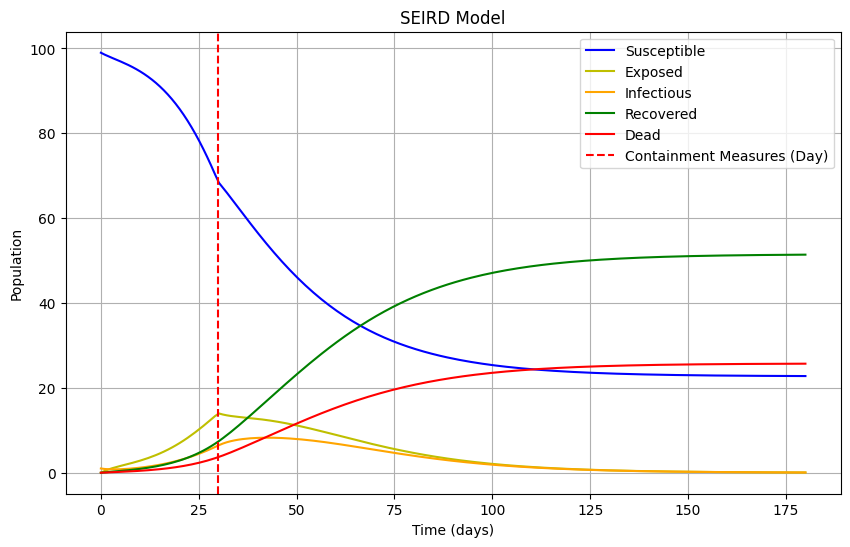
\includegraphics[width=0.5\textwidth]{ContainmentA.png}
    \caption{Simulation w/ Containment Effectiveness = 0.9.}
    \label{ContainmentA}
\end{figure}
\begin{figure}
    \centering
    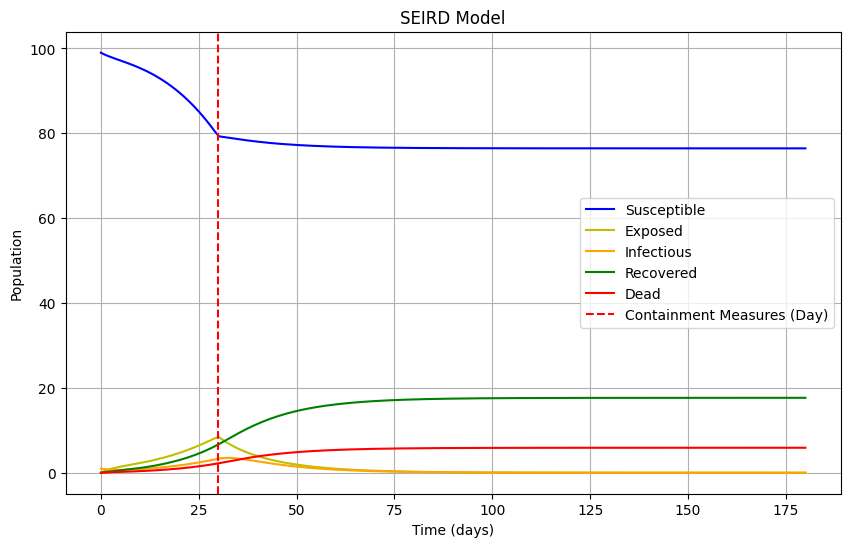
\includegraphics[width=0.5\textwidth]{ContainmentB.png}
    \caption{Simulation w/ Containment Effectiveness = 0.5.}
    \label{ContainmentB}
\end{figure}
\begin{figure}
    \centering
    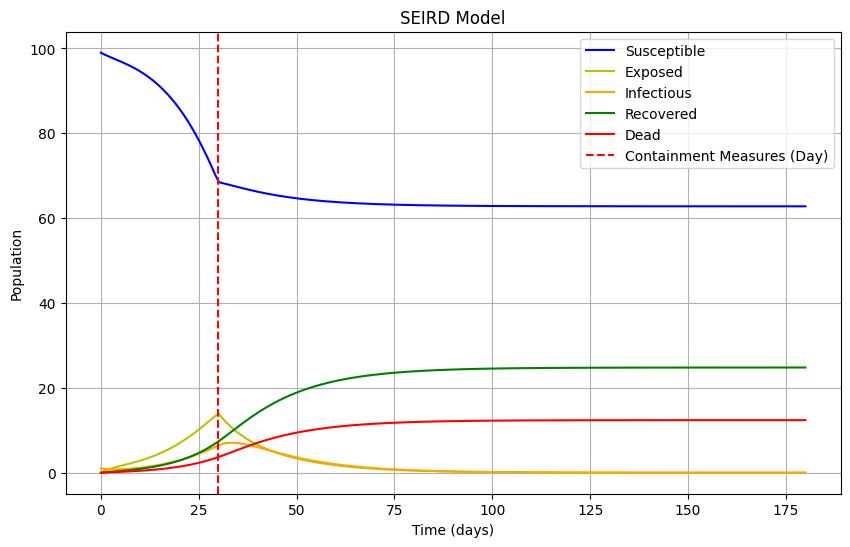
\includegraphics[width = 0.5\textwidth]{ContainmentC.png}
    \caption{Simulation w/ Containment Effectiveness = 0.1.}
    \label{ContainmentC}
\end{figure}

\subsection{Impact of Combining Healthcare and Containment Measures}
\textcolor{blue}{
    Finally, I ran even more simulations to understand the impact of combining healthcare and containment measures on the spread of the disease.
    I used the same parameters as in the previous simulations, but played around with the healthcare quality and containment effectiveness parameters until I found a combination that seemed to work best.
    I found that the combination of 0.66 healthcare quality and 0.66 containment effectiveness (figure 9) seemed to work best, with a final death count of only 7.}
\section{Discussion and Conclusions}
\begin{figure}
    \centering
    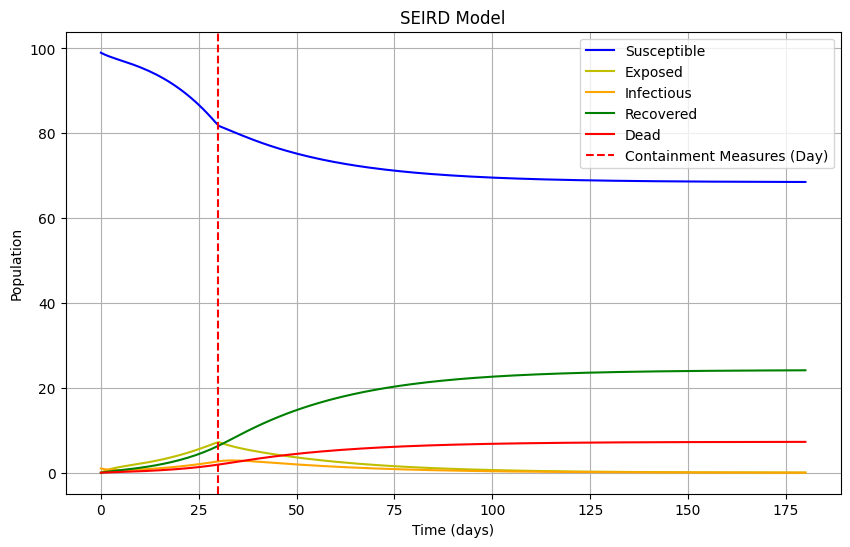
\includegraphics[width=0.5\textwidth]{bestcombo.png}
    \caption{Simulation w/ Healthcare Quality = 0.66 and Containment Effectiveness = 0.66.}
    \label{Best Combo}
\end{figure}

\subsection{Mapping with Geospatial Data}
\textcolor{blue}{
    I also tried to collect geospatial data on countries and cities affected by the Ebola epidemic in West Africa.
    This was accomplished using the python libaries geopandas and folium.
    I loaded in a shapefile of the countries in West Africa, and then plotted the coordinates of the affected cities on the map.
    This allowed me to visualize the spread of the disease in a more interactive way.
    I also attempted to create an animation of the spread of the disease using the SEIRD model, but was unable to get it to work.
    This is something I would like to work on in the future.
    The maps I created can be seen in figures 10 and 11.}
\begin{figure}
    \centering
    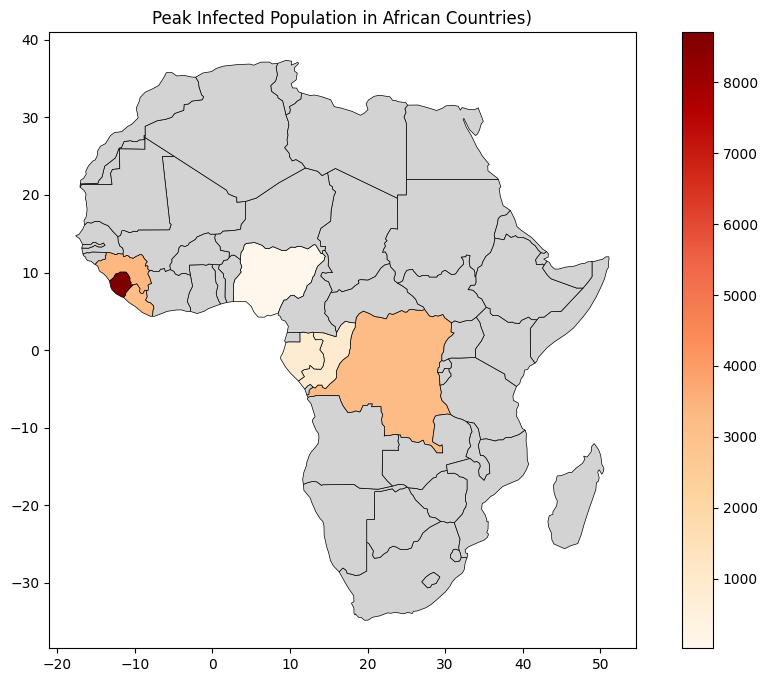
\includegraphics[width=0.5\textwidth]{PeakInfectedAfrica.png}
    \caption{Map of the Ebola Epidemic in West Africa.}
    \label{Ebola Map}
\end{figure}
\begin{figure}
    \centering
    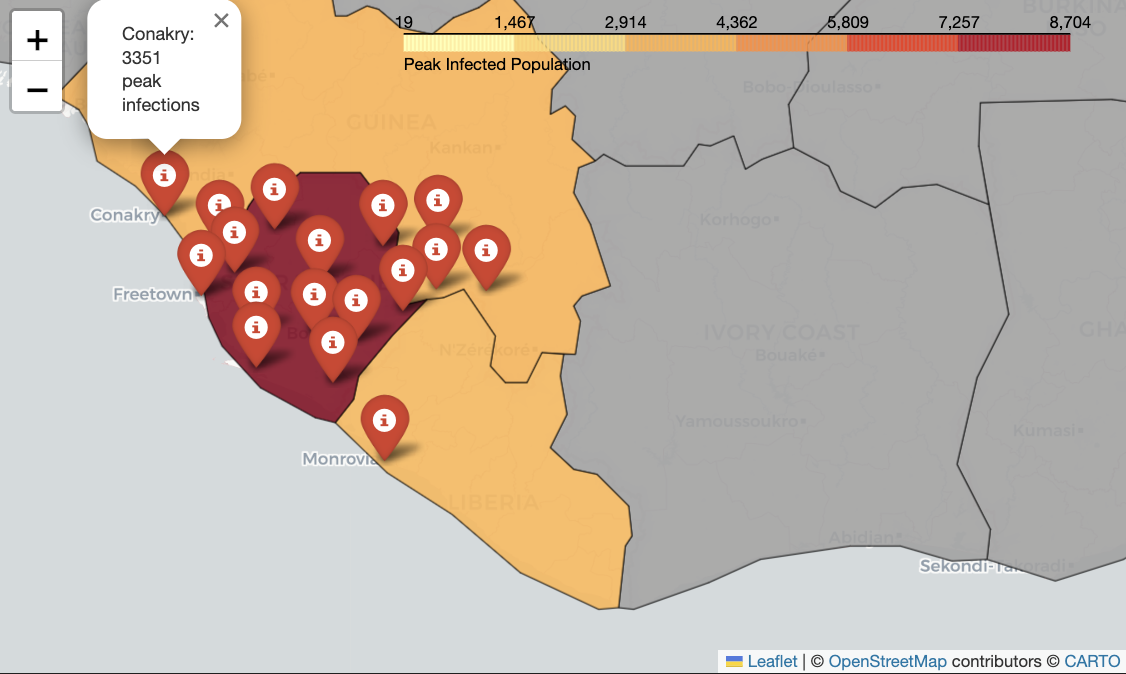
\includegraphics[width=0.5\textwidth]{InteractiveMap.png}
    \caption{Map of the Ebola Epidemic in West Africa.}
    \label{Ebola Map}
\end{figure}

Finally: Which of your findings surprised you? What were your favorite discoveries and why? 

\textcolor{blue}{
        Upon running various simulations using an SEIRD model to simulate the spread of Ebola, 
    I noticed that the both quality of healthcare and the effectiveness of containment measures had a significant impact on controlling the epidemic.
    The disease spread more slowly and had less total fatalitites when either healthcare quality was high or containment measures were effective. 
    I also found that the combination of healthcare and containment measures was and even more effective method of controlling the disease.
    Lastly, I also tested various intital containment dates and found that the earlier the containment measures were implemented, the more effective they were,
    while the later the containment measures were implemented, the less effective they were. This was a key finding in my project.
    This highlights the importance of healthcare, containment measures and timely containment in controlling the spread of infectious diseases.
}
\textcolor{blue}{
    I would ultimately say that my project has been successful in achieving my learning goals.
    I was successfully able to model the theoretical spread of Ebola using a custom SEIRD model.
    In the process, I came to learn much about the dynamics of infectious diseases and how they can be modeled.
    It also reinforced my understanding of the importance of healthcare and containment measures in controlling the spread of disease.
    Arguably the most important thing I gained from this was experience in data collection and analysis, as well as geospatial analysis.
}
\section{Outlook and Future Work}
\textcolor{blue}{
    This has been a great experience and as I move forward I would like to continue to do this type of research. If I had more time to work on this project,
    I would like to refine my model even further and test it on more real-world data.
    I believe the model is missing the ability for deceased individuals to infect others, which is a key feature of diseases such as Ebola.
    It is also somewhat unrealistic how the containment measures are implemented in the model, happening instantly instead of gradually.
    Often times, containment measures are implemented gradually, and I would like to account for this in my model.
    Some of the things I considered adding to my model were the effects of population density and age distribution.
    It would be interesting to make a predictive model that could be used to forecast the spread of Ebola in the future.
    Ultimately, I plan to continue to work on the geospatial mapping I did in this project. I want my maps to be more interactive and to be able to run an animation of the spread of the disease using my model.
    }

\newpage
\begin{thebibliography}{2}

\bibitem{aa} Caitlyn Rivers, 2014, https://github.com/cmrivers/ebola.

\bibitem{bb} World Health Organization, 2014, https://www.who.int/csr/disease/ebola/en/

\bibitem{cc} Centers for Disease Control and Prevention, 2014, https://www.cdc.gov/vhf/ebola/index.html

\end{thebibliography}

\end{document}
%
% ****** End of file apssamp.tex ******
